\chapter{Aufgabe 1}

\section{Teil 1}
\textit{Welcher Bootlader sitzt auf dem Image?}\\

\noindent
Wie dem Hexdump~\ref{lst:hexdump} zu entnehmen ist, handelt es sich bei den ersten 512 Bytes der Datei um einen gültigen Bootblock, erkennbar an den letzten beiden Bytes $0x55$ und $0xAA$ (\textit{Signatur}, vgl.~\cite[142]{ES4}).\\
Der \textbf{Bootloadername} ist in den ersten 11 Bytes zu finden: Es handelt sich um den Bootloader \texttt{Syslinux}\footnote{
\url{https://en.wikipedia.org/wiki/SYSLINUX}, abgerufen 09.04.2025
}.

\vspace{5mm}

\begin{lstlisting}[caption={Hexdump der ersten 512 Bytes der Datei \textasciitilde{}/Einsendeaufgaben/ESA1/ImageESA1.flp} (Ausschnitt), captionpos=b, label={lst:hexdump},basicstyle=\ttfamily\footnotesize, frame=single]
00000000  eb 58 90 53 59 53 4c 49  4e 55 58 00 02 04 04 00  ; .X.SYSLINUX••••
00000010  02 00 02 10 27 f8 08 00  20 00 40 00 00 00 00 00  ; ••••'.•• @@00000
.
.
.
000001e0  72 72 6f 72 0d 0a 00 00  00 00 00 00 00 00 00 00  ; rror__00 00000000
000001f0  00 00 00 00 00 00 00 00  fe 02 b2 3e 18 37 55 aa  ; 00000000.•.>•7U.
00000200  00 00 00 00 00 00 00 00  00 00 00 00 00 00 00 00  ; 00000000 00000000
\end{lstlisting}


\section{Teil 2}

\textit{Wie heißt die  \texttt{initrd} des Image?}\\

\noindent
Wir können wahlweise mit den in dem Verzeichnis vorhandenen Tool \texttt{imgm} das Image mounten und uns den Verzeichnisinhalt anschauen, oder uns mittels \texttt{imgls} den Inhalt der Image-Datei anzeigen lassen  (siehe Listing~\ref{lst:imgls}) - in beiden Fällen werden wir auf die Datei \texttt{hello.ird} stoßen, die die \texttt{initrd} des Image repräsentiert.\\
Wir überprüfen den Inhalt von \texttt{syslinux.cfg} (Konfigurationsdatei für den geg. Bootloader) und finden:

\begin{verbatim}
default linux
append clock=pit rw  initrd=hello.ird
display banner
timeout 0
\end{verbatim}

\noindent
was den Namen der \texttt{initrd} bestätigt.

\vspace{5mm}

\begin{lstlisting}[
caption={Inhalt des Images ImageESA1.flp (erzeugt mit imgls)},
captionpos=b,
label={lst:imgls},
basicstyle=\ttfamily\footnotesize,
frame=single,
keepspaces=true,
showspaces=false
]
   2 -rwxr-xr-x 1 root root    1659 Feb 16  2023 banner
 312 -rwxr-xr-x 1 root root  318154 Feb 16  2023 hello.ird
  32 -r-xr-xr-x 1 root root   32768 Sep  8  2017 ldlinux.sys
2456 -rwxr-xr-x 1 root root 2513024 Sep  8  2017 linux
   2 -rwxr-xr-x 1 root root      77 Jan 23  2023 syslinux.cfg
\end{lstlisting}


\section{Teil 3}

\textit{Wie ist die \texttt{initrd} des Image gepackt worden?}\\

\noindent
In~\cite[112]{ES4} wird das (ursprüngliche) Konzept\footnote{
``Das Konzept der initrd wurde mit der Kernelversion 2.6 stark überarbeitet.
Die initrd kann vollständig durch den Nachfolger initramfs ersetzt werden [\ldots]`` (\textit{ebd.})
} der \textit{Initial Ram Disk} beschrieben, wo es u.a. heißt, dass \texttt{gzip} zum Packen verwendet wird.
Ein Aufruf von

\begin{center}
\texttt{file hello.ird}
\end{center}

\noindent
zeigt auch für \underline{diese Datei} (s. nachfolgende Aufgabe zur Einschränkung hinsichtlich \texttt{initrd}):\\

\noindent
\texttt{hello.ird: gzip compressed data, from Unix, original size modulo 2\^32 710144}

\section{Teil 4}

\textit{Welche Datei der \texttt{initrd} ist gestartet worden?}\\

\noindent
In der Datei \texttt{hello.ird} finden wir die Datei \texttt{hello} - eine Überprüfung mittels

\begin{center}
    \texttt{file hello}
\end{center}

\noindent
liefert

\begin{verbatim}
hello: ASCII cpio archive (SVR4 with no CRC)
\end{verbatim}

\noindent
Mit~\cite[117 f.]{ES4} können wir also annehmen, dass wir es hier mit einer \texttt{initramfs} zu tun haben.\\
Weiteres Entpacken des \texttt{cpio}-Archiv liefert die Datei \texttt{init}, eine Überprüfung mit \texttt{file} liefert:

\begin{verbatim}
init: ELF 32-bit LSB executable, Intel 80386, version 1 (GNU/Linux),
statically linked, BuildID[sha1]=c549239ca2a5ae08c25bdf841ee2e2bb09891cde,
for GNU/Linux 3.2.0, not stripped
\end{verbatim}

\noindent
Hierbei handelt es sich also um eine \textit{Executable and Linkable Format}-Datei (\cite[24]{ES4}), welche gestartet wird (siehe nachfolgende Aufgabe).

\section{Teil 5}

\textit{Starten Sie das System mit \texttt{QEMU}. Welche Meldung gibt das Anwendungsprogramm aus?}\\

\noindent
Es wird die Meldung \texttt{Hallo Welt} ausgegeben (s. Abb.~\ref{fig:qemus}).

\begin{figure}
\centering
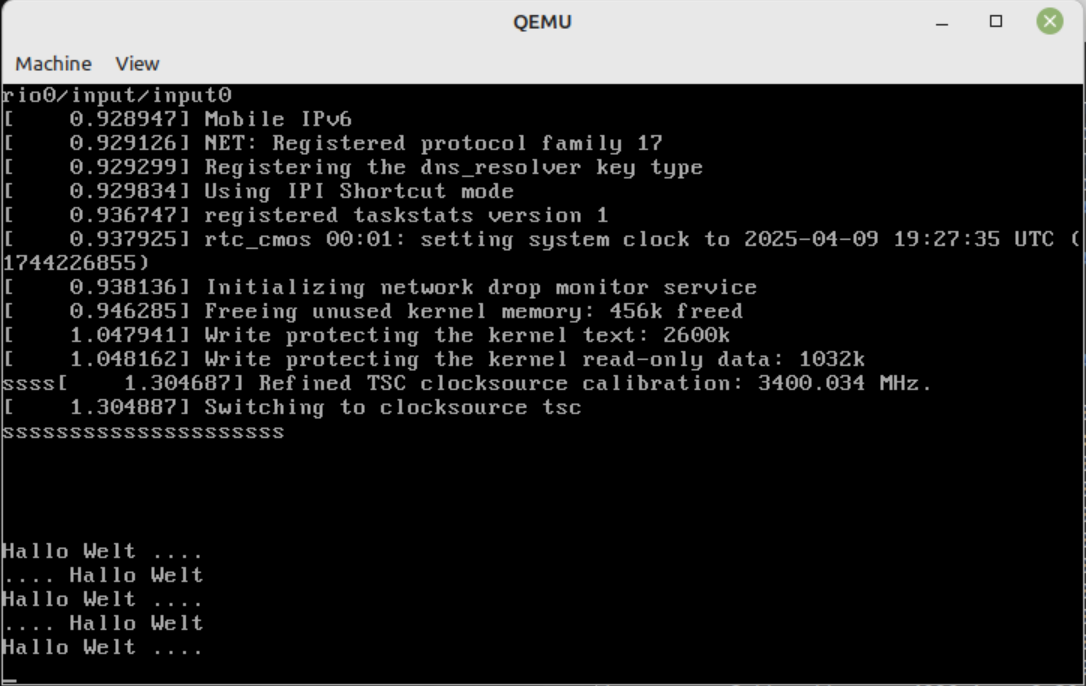
\includegraphics[scale=0.3]{aufgabe 1/img/qemus}
\caption{Screenshot der Bildschirmausgabe nach dem Aufruf von \texttt{qemus ./ImageESA1.flp}  (Quelle: eigene)}
\label{fig:qemus}
\end{figure}
